\documentclass[tikz,border=5pt]{standalone}
\usetikzlibrary{positioning, fit, backgrounds, calc}

% ── Palette ────────────────────────────────────────────────────
\definecolor{canvadark}{HTML}{0D1B2A}

\definecolor{clIDE}   {HTML}{065F46}
\definecolor{clAPI}   {HTML}{92400E}
\definecolor{clORCH}  {HTML}{9D174D}
\definecolor{clMEM}   {HTML}{3B4A6B}
\definecolor{clAGENT} {HTML}{1E3A5F}
\definecolor{clINF}   {HTML}{7F1D1D}

\definecolor{bIDE}    {HTML}{00C9B1}
\definecolor{bAPI}    {HTML}{F59E0B}
\definecolor{bORCH}   {HTML}{EC4899}
\definecolor{bMEM}    {HTML}{94A3B8}
\definecolor{bAGENT}  {HTML}{3B82F6}
\definecolor{bINF}    {HTML}{EF4444}
% ───────────────────────────────────────────────────────────────

\begin{document}
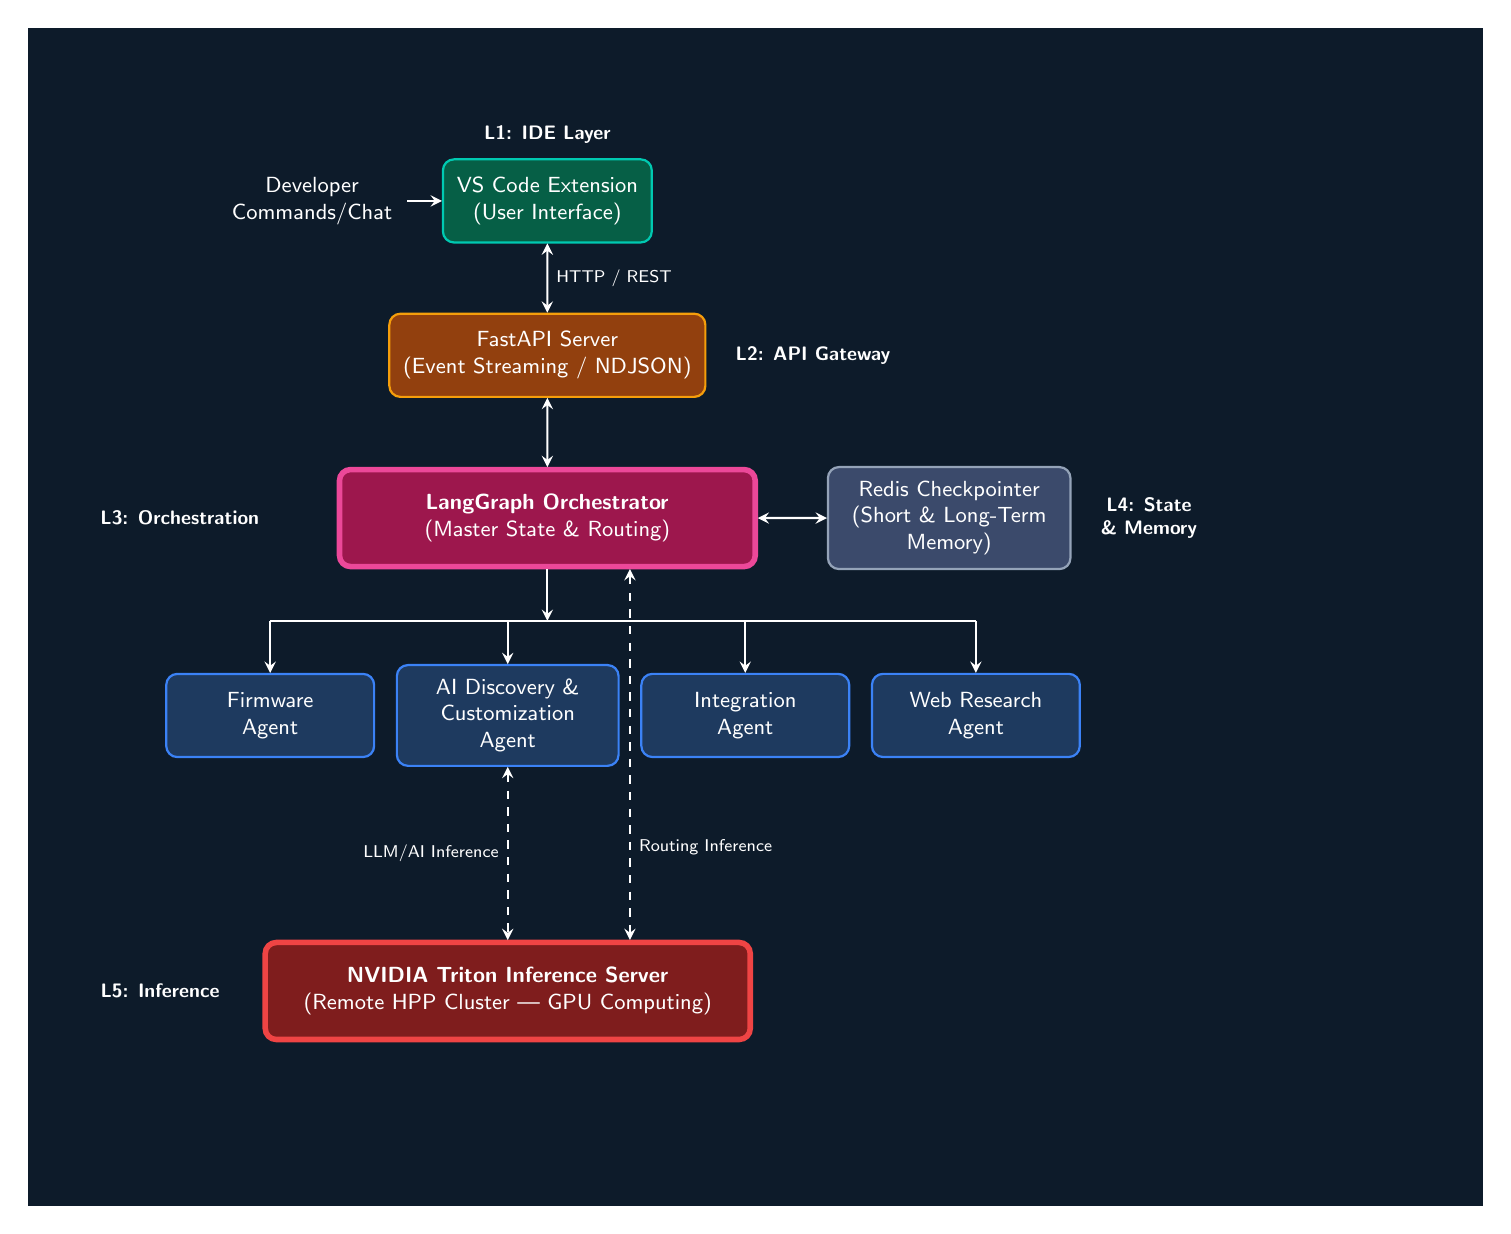
\begin{tikzpicture}[
    scale=0.88, transform shape,
    node distance=1.5cm and 1.8cm,
    every node/.style={font=\sffamily\small, text=white},
    box/.style={
        draw, rounded corners,
        minimum width=3cm, minimum height=1.2cm,
        align=center, thick, inner sep=0.2cm, text=white
    },
    corebox/.style={
        draw, rounded corners,
        minimum width=6cm, minimum height=1.4cm,
        align=center, line width=2pt, inner sep=0.2cm, text=white
    },
    arrow/.style={->, thick, >=stealth, draw=white},
    dblarrow/.style={<->, thick, >=stealth, draw=white},
    layerlabel/.style={
        font=\sffamily\footnotesize\bfseries,
        text=white, align=center
    }
]

% ── BACKGROUND ─────────────────────────────────────────────────
\begin{scope}[on background layer]
    \fill[canvadark] (-7.5, 2.5) rectangle (13.5, -14.5);
\end{scope}

% ── LAYER 1: IDE ───────────────────────────────────────────────
\node[box, fill=clIDE, draw=bIDE] (vscode)
    {VS Code Extension \\ (User Interface)};

\node[layerlabel, above=0.1cm of vscode] {L1: IDE Layer};

\node[left=0.5cm of vscode, align=center,
      text width=2.5cm, text=white] (user)
    {Developer \\ Commands/Chat};
\draw[arrow] (user) -- (vscode);

% ── LAYER 2: API Gateway ───────────────────────────────────────
\node[box, fill=clAPI, draw=bAPI,
      below=1cm of vscode] (fastapi)
    {FastAPI Server \\ (Event Streaming / NDJSON)};

\draw[dblarrow] (vscode) --
    node[right, font=\sffamily\scriptsize]{HTTP / REST}
    (fastapi);

\node[layerlabel, right=0.3cm of fastapi] {L2: API Gateway};

% ── LAYER 3: Orchestration ─────────────────────────────────────
\node[corebox, fill=clORCH, draw=bORCH,
      below=1cm of fastapi] (langgraph)
    {\textbf{LangGraph Orchestrator} \\ (Master State \& Routing)};

\draw[dblarrow] (fastapi) -- (langgraph);

\node[layerlabel, left=1cm of langgraph] {L3: Orchestration};

% ── LAYER 4: State & Memory ────────────────────────────────────
\node[box, fill=clMEM, draw=bMEM,
      right=1cm of langgraph, minimum width=3.5cm] (redis)
    {Redis Checkpointer \\ (Short \& Long-Term \\ Memory)};

\draw[dblarrow] (langgraph.east) -- (redis.west);

\node[layerlabel, anchor=west] at ([xshift=0.3cm]redis.east)
    {L4: State \\ \& Memory};

% ── AGENTS ─────────────────────────────────────────────────────
\node[box, fill=clAGENT, draw=bAGENT,
      below=1.5cm of langgraph, xshift=-4cm,
      text width=2.4cm] (fw_agent)
    {Firmware \\ Agent};

\node[box, fill=clAGENT, draw=bAGENT,
      right=0.3cm of fw_agent, text width=2.8cm] (ai_agent)
    {AI Discovery \& \\ Customization \\ Agent};

\node[box, fill=clAGENT, draw=bAGENT,
      right=0.3cm of ai_agent, text width=2.4cm] (int_agent)
    {Integration \\ Agent};

\node[box, fill=clAGENT, draw=bAGENT,
      right=0.3cm of int_agent, text width=2.4cm] (web_agent)
    {Web Research \\ Agent};

% Bus orizzontale → agenti
\coordinate (bus) at ([yshift=-0.75cm]langgraph.south);
\draw[arrow] (langgraph.south) -- (bus);
\draw[white, thick]
    (fw_agent.north |- bus) -- (web_agent.north |- bus);
\draw[arrow] (bus -| fw_agent.north)  -- (fw_agent.north);
\draw[arrow] (bus -| ai_agent.north)  -- (ai_agent.north);
\draw[arrow] (bus -| int_agent.north) -- (int_agent.north);
\draw[arrow] (bus -| web_agent.north) -- (web_agent.north);

% ── LAYER 5: Inference ─────────────────────────────────────────
\node[corebox, fill=clINF, draw=bINF,
      below=2.5cm of ai_agent, minimum width=7cm] (triton)
    {\textbf{NVIDIA Triton Inference Server} \\
     (Remote HPP Cluster --- GPU Computing)};

\node[layerlabel, left=0.5cm of triton] {L5: Inference};

% ── FRECCE TRATTEGGIATE verso Triton ───────────────────────────

% LLM/AI Inference: da ai_agent a Triton (label a sinistra)
\draw[dblarrow, dashed]
    (ai_agent.south) --
    node[left, font=\sffamily\scriptsize]{LLM/AI Inference}
    (triton.north -| ai_agent.south);

% Routing Inference: punto medio tra ai_agent.east e int_agent.west
% freccia verticale da langgraph.south a triton.north (label a destra)
\path (ai_agent.east) -- (int_agent.west)
    coordinate[midway] (mid_ai_int);
\draw[dblarrow, dashed]
    (langgraph.south -| mid_ai_int) --
    node[right, near end, font=\sffamily\scriptsize]{Routing Inference}
    (triton.north -| mid_ai_int);

\end{tikzpicture}
\end{document}
